%&../settings/preamble.main

\ifsubfile
\pagestyle{plain}
\setcounter{chapter}{18}

% arara: pdflatex: { options: ["--output-directory=../build"], draft: yes, synctex: no }
% arara: pdflatex: { options: ["--output-directory=../build"], synctex: no }
\begin{document}
\fi
\chapter{Soluzioni per problemi intrattabili}
\epigraph{Chi si accontenta, gode}{Proverbio}

\section{Algoritmi pseudo-polinomiali}

Non si può avere tutto dalla vita; bisogna rinunciare a qualcosa:
\begin{itemize}
	\item \textbf{generalità}: algoritmi \alert{pseudo-polinomiali} che funzionano per solo alcuni casi particolari dell'input;
	\item \textbf{ottimalità}: algoritmi di \alert{approssimazione}, che garantiscono di ottenere soluzioni \enquote{vicine} alla soluzione ottimale;
	\item \textbf{formalità}: algoritmi \alert{euristici}, di solito basati su tecniche \foreign{greedy} o di ricerca locale, che forniscano sperimentalmente risultati buoni;
	\item \textbf{efficienza}: algoritmi esponenziali \alert{branch-\&-bound}, che limitano lo spazio di ricerca con un'accurata potatura.
\end{itemize}
Per il rilassamento di ognuno di questi vincoli possiamo definire un tecnica.

\subsection{Somma di sottoinsiemi {\subSetSumProblem}}

\paragraph{Definizione del problema}
Dati un insieme \(A = \{a_1, a_2, \dots, a_n\}\) di interi positivi e un intero positivo \(k\), \alert{esiste} un sottoinsieme \(S\) di indici in \(\{1, \dots, n\}\) tale che \(\sum_{i \in S} A_i = k\) ?

Utilizzando \foreign{backtracking}, abbiamo risolto la versione di ricerca di questo problema.
Quella appena enunciata è la versione decisionale.
Per semplificare il confronto, ci concentriamo sulla seconda.

\subsubsection{Somma di sottoinsiemi risolto tramite programmazione dinamica}

Definiamo una tabella booleana \(DP[0 \dots n][0 \dots k]\).
\(DP[i][r]\) è uguale a \True se esiste un sottoinsieme dei primi \(i\) valori memorizzati in \(A\) la cui somma è pari a \(r\), \False altrimenti.
Il problema generale è definito da \(DP[n][k]\).

\paragraph{Definizione dell'equazione di ricorrenza}
Analizziamo caso per caso.
Prima i casi base:
\begin{itemize}
	\item[\circled{1}] se devo ottenere un valore uguale a \(0\) (\(r=0\)), sono sicuro che non prendendo nessun oggetto posso ottenere quel valore, quindi restituiremo \True;

	\item[\circled{2}] nel caso in cui voglia ottenere un valore (\(r>0\)), ma non ho più alcun oggetto da sommare (\(i=0\)), allora non mi sarà possibile soddisfare la richiesta, restituirò \False.
\end{itemize}

Consideriamo ora i casi in cui vogliamo ottenere un valore (\(r>0\)) e abbiamo ancora oggetti a nostra disposizione (\(i>0\)).

\begin{itemize}[resume]
	\item[\circled{3}] il valore dell'oggetto considerato è troppo grande rispetto al valore \(r\) che voglio ottenere (\(A[i] > r\)), quindi escludo quell'oggetto (\(i-1\)) e lascio inalterato il valore \(r\);

	\item[\circled{4}] posso prendere anche l'ultimo oggetto in quanto il suo valore non eccede \(r\) (\(A[i] \leqslant r\)), quindi considero la possibilità di non prenderlo e di lasciare inalterato il valore di \(r\) (\(DP[i - 1][r]\)), oppure lo prendo e sottraggo il suo valore a quello che voglio ottenere (\(DP[i - 1][r - A[i]]\)).
\end{itemize}
Siamo quindi riusciti a definire l'equazione di ricorrenza come segue
\[
	DP[i][r] =
	\begin{dcases}
		\True                                         & r = 0 \\
		\False                                        & r > 0 \land i = 0\\
		DP[i-1][r]                                    & r > 0 \land i > 0 \land A[i] > r\\
		DP[i - 1][r] \text{ \Or } DP[i - 1][r - A[i]] & r > 0 \land i > 0 \land A[i] \leqslant r\\
	\end{dcases}
\]

L'algoritmo sfrutta l'equazione di ricorrenza.
\begin{algorithm}[H]
	\caption{Somma di sottoinsiemi risolto tramite programmazione dinamica}
	%&../preamble

% arara: pdflatex: { synctex: no }
% arara: latexmk: { clean: partial }
\ifstandalone
\begin{document}
\begin{algorithm}[H]
\fi

\prototype{\Bool \subSetSum{\Array{\Int} \(A\), \Int \(n\), \Int \(k\)}}{

	\BlankLine
	\Matrix{\Bool} \(DP\) \Assign \new \Matrix{\Bool}[0\dots n][0\dots k] = \{{\False}\}\;

	\BlankLine
	\tcp{CASI BASE}

	\BlankLine
	\tcp{se il valore da ottenere è 0, non ho bisogno di selezionare nessun indice}
	\For(\tcp*[h]{\(prima colonna\)}){\(i \Assign 0\) \DownTo \(n\)}{

		\BlankLine
		\(DP[i][0] \Assign \True\) \tcp{\(r=0\)}
	}

	\BlankLine
	\tcp{se non ho nessun intero positivo da selezionare non mi è possibile arrivare al valore richiesto}
	\For(\tcp*[h]{\(prima riga\)}){\(r \Assign 1\) \DownTo \(k\)}{

		\BlankLine
		\(DP[0][r] \Assign \False\) \tcp{\(r>0 \land i=0\)}
	}

	\BlankLine
	\tcp{CASO RICORSIVO}
	\From{\(i \Assign 1\) \DownTo \(n\)}{
		\From(\tcp*[h]{\(commento\)}){\(r \Assign 1\) \DownTo \(A[i]-1\)}{

			\BlankLine
			\(DP[i][r] \Assign DP[i-1][r]\) \tcp{\(A[i] > r\)}
		}

		\BlankLine
		\From(\tcp*[h]{\(commento\)}){\(r \Assign A[i]\) \DownTo \(k\)}{

			\BlankLine
			\(DP[i][r] \Assign DP[i-1][r]\) \Or \(DP[i-1][r - A[i]]\) \tcp{\(A[i] \leqslant r\)}
		}
	}

	\BlankLine
	\tcp{restituisco il valore in posizione \(k\)-esima}
	\Return \(DP[n][k]\)\;
}

\ifstandalone
\end{algorithm}
\end{document}
\fi

\end{algorithm}

\paragraph{Complessità}
Essendo un problema decisionale, è possibile semplificare e utilizzare spazio \(\Theta(k)\), invece che \(\Theta(nk)\), in quanto avrò \(n\) righe e \(k\) colonne.

\paragraph{Esempio di esecuzione}
Ad esempio prendendo l'insieme \(A = [5,9,10]\) di interi positivi e l'intero positivo \(k = 24\) proviamo a riempire la tabella di programmazione dinamica.
Dove le righe rappresentano il numero di oggetti presi e le colonne il valore di \(k\) desiderato.

{
\setlength{\tabcolsep}{3pt}
\begin{tabularx}{\textwidth}{@{} l *{25}{ F{Y} } c @{}}
	\toprule
		& \textbf{0} & \textbf{1} & \textbf{2} & \textbf{3} & \textbf{4} & \textbf{5} & \textbf{6} & \textbf{7} & \textbf{8} & \textbf{9} & \textbf{10} & \textbf{11} & \textbf{12} & \textbf{13} & \textbf{14} & \textbf{15} & \textbf{16} & \textbf{17} & \textbf{18} & \textbf{19} & \textbf{20} & \textbf{21} & \textbf{22} & \textbf{23} & \textbf{24} & \emph{A}\\
	\cmidrule{2-26}
		\textbf{0} & 1 &&&&&&&&&&&&&&&&&&&&&&&&\\
	\lightrule
		\textbf{1} & 1 &&&&& 1 &&&&&&&&&&&&&&&&&&&& \textbf{5}\\
	\lightrule
		\textbf{2} & 1 &&&&& 1 &&&& 1 &&&&& 1 &&&&&&&&&&& \textbf{9}\\
	\lightrule
		\textbf{3} & 1 &&&&& 1 &&&&1 & 1 &&&& 1 & 1 &&&& 1 &&&&& 1& \textbf{10}\\
	\bottomrule
\end{tabularx}
}

\paragraph{Analisi della complessità}
La complessità dell'algoritmo è \(\Theta(nk)\), ma la complessità dei dati in ingresso è \(\Omicron(n \log k)\), in quanto i valori più grandi del nostro obiettivo possono essere esclusi.
Se \(k\) è \(\Omicron(n^c)\) con \(c\) costante, allora \subSetSum ha complessità polinomiale \(\Omicron(n^{c+1})\).
Ma se \(k\) è  \(\Omicron(2^n)\), allora \subSetSum ha complessità superpolinomiale \(\Omicron(n \cdot 2^{n})\).

\begin{observation}
La complessità di \subSetSum dipende quindi dai valori contenuti nell'insieme e non soltanto dalla cardinalità dei dati in ingresso (\(n\)).
\end{observation}

\subsubsection{Somma di sottoinsiemi risolto tramite backtracking}

\begin{algorithm}[H]
	\caption{Somma di sottoinsiemi risolto tramite backtracking}
	%&../preamble

% arara: pdflatex: { synctex: no }
% arara: latexmk: { clean: partial }
\ifstandalone
\begin{document}
\begin{algorithm}[H]
\fi

\prototype{\Bool \subSetSumRec{\Array{Int} \(A\), \Int \(i\), \Int \(r\)}}{

	\BlankLine
	\uIf{\(r \Equal 0\)}{
		\Return \True\;
		\BlankLine
	}
	\uElseIf{\(i \Equal 0\)}{
		\Return \False\;
		\BlankLine
	}
	\uElseIf{\(A[i] > r\)}{
		\Return \(\subSetSumRec(A, i-1, r)\)\;
		\BlankLine
	}
	\Else{
		\Return \(\subSetSumRec(A, i-1, r)\) \Or \(\subSetSumRec(A, i-1, r-A[i])\)\;
	}

	\BlankLine
	\Return \(res\)\;
}

\ifstandalone
\end{algorithm}
\end{document}
\fi

\end{algorithm}

\paragraph{Esempio di esecuzione}
Prendiamo sempre in considerazione l'insieme \(A = [5,9,10]\) di interi positivi e l'intero positivo \(k = 24\).
In questo caso non viene effettivamente calcolata una tabella, in quanto sono tutte chiamate ricorsive, ma viene riportata per comodità.
Dove le righe rappresentano il numero di oggetti presi \(i\) e  le colonne il valore di \(r\).
Ad esempio per calcolare la chiamata (\(i=3\), \(r=24\)) vengono calcolati ricorsivamente il caso precedente (\(i-1 = 3-1 = 2, r = 24\)) e il caso (\(i-1 = 3-1 = 2\), \(r-A[i] = 24-10 = 14\)), ricorsivamente per calcolare (\(i=2, r=24\)) viene effettuata la chiamata ricorsiva per calcolare il caso precedente (\(i-1 = 2-1 = 1\), \(r = 14\)) e il caso (\(i-1 = 2-1 = 1\), \(r = r-A[i] = 14-9 = 5\)).

{
\setlength{\tabcolsep}{3pt}
\begin{tabularx}{\textwidth}{@{} l *{25}{ F{Y} } c @{}}
	\toprule
		& \textbf{0} & \textbf{1} & \textbf{2} & \textbf{3} & \textbf{4} & \textbf{5} & \textbf{6} & \textbf{7} & \textbf{8} & \textbf{9} & \textbf{10} & \textbf{11} & \textbf{12} & \textbf{13} & \textbf{14} & \textbf{15} & \textbf{16} & \textbf{17} & \textbf{18} & \textbf{19} & \textbf{20} & \textbf{21} & \textbf{22} & \textbf{23} & \textbf{24} & \emph{A}\\
	\cmidrule{2-26}
		\textbf{0} & 1 &&&&& 0 &&&& 0 & 0 &&&& 0 & 0 &&&&&&&&& 0 & \\
	\lightrule
		\textbf{1} &&&&&& 1 &&&&&&&&& 0 & 0 &&&&&&&&& 0 & \textbf{5}\\
	\lightrule
		\textbf{2} &&&&&&&&&&&&&&& 1 &&&&&&&&&& 0 & \textbf{9}\\
	\lightrule
		\textbf{3} &&&&&&&&&&&&&&&&&&&&&&&&& 1 & \textbf{10}\\
	\bottomrule
\end{tabularx}
}

\paragraph{Complessità}
Ognuno dei valori è stato calcolato tramite chiamate ricorsive.
Una chiamata ricorsiva quando \(i=3\), due chiamate ricorsive quando \(i=2\), quattro chiamate ricorsive quando \(i=1\) ed infine otto chiamate quando \(i=0\).
Il che è ovvio visto che abbiamo usato un algoritmo esponenziale e quindi raddoppio le chiamate ad ogni passo.
Per una complessità totale di \(\Omicron(2^n)\).

\subsubsection{Somma di sottoinsiemi risolto tramite memoization}

\begin{algorithm}[H]
	\caption{Somma di sottoinsiemi risolto tramite memoization}
	%&../preamble

% arara: pdflatex: { synctex: no }
% arara: latexmk: { clean: partial }
\ifstandalone
\begin{document}
\begin{algorithm}[H]
\fi

\prototype{\Bool \subSetSumMemo{\Array{\Int} \(A\), \Int \(i\), \Int \(r\), \dictionary \(\DP\)}}{

	\BlankLine
	\tcp{CASI BASE}
	\uIf{\(r \Equal 0\)}{
		\Return \True\;
		\BlankLine
	}
	\uElseIf{\(r < 0\) \Or \(i \Equal 0\)}{
		\Return \False\;
	}
	\Else(\tcp*[h]{CASI RICORSIVI}){
		\Bool \(\result\) \Assign \(\DP.\dictLookup((i,r))\) \tcp{uso come chiave la descrizione del problema}

		\BlankLine
		\If(\tcp*[h]{se il problema non è stato ancora calcolato}){\(res \Equal \Nil\)}{


			\BlankLine
			\(\result\) \Assign \subSetSumMemo{\(A\), \(i-1\), \(r\), \(\DP\)} \tcp{calcolo il caso precedente}

			\BlankLine
			\If(\tcp*[h]{se posso prenderlo prendo in considerazione la possibilità di farlo}){\(A[i] < r\)}{
				\(\result\) \Assign \(\result\) \Or \(\subSetSumMemo(A, i-1, r-A[i], DP)\)\;
			}

			\BlankLine
			\(DP.\dictInsert((i,r), res)\) \tcp{inserisco la soluzione nel dizionario}
		}

		\BlankLine
		\Return \(\result\)\;
	}
}

\ifstandalone
\end{algorithm}
\end{document}
\fi

\end{algorithm}

\paragraph{Complessità}
Il dizionario viene rappresentano come una tabella, ma potrebbe essere una \enquote{hashtable}.

Se proviamo a riproviamo ad applicare questo algoritmo sull'esempio precedente, le caselle del dizionario che verranno riempite sono solo quelle contenenti i problemi da risolvere e non tutti.
Nel caso ci siano molti problemi ripetuti il caso pessimo è rappresentato dalla complessità \(\Omicron(nk)\), ossia il caso in cui dobbiamo per forza riempire tutto il dizionario.

{
\setlength{\tabcolsep}{3pt}
\begin{tabularx}{\textwidth}{@{} l *{25}{ Y } c @{}}
	\toprule
		& \textbf{0} & \textbf{1} & \textbf{2} & \textbf{3} & \textbf{4} & \textbf{5} & \textbf{6} & \textbf{7} & \textbf{8} & \textbf{9} & \textbf{10} & \textbf{11} & \textbf{12} & \textbf{13} & \textbf{14} & \textbf{15} & \textbf{16} & \textbf{17} & \textbf{18} & \textbf{19} & \textbf{20} & \textbf{21} & \textbf{22} & \textbf{23} & \textbf{24} & \emph{A}\\
	\cmidrule{2-26}
		\textbf{0} & 1 &&&&& 0 &&&& 0 & 0 &&&& 0 & 0 &&&&&&&&& 0 & \\
	\lightrule
		\textbf{1} &&&&&& 1 &&&&&&&&& 0 & 0 &&&&&&&&& 0 & \textbf{5}\\
	\lightrule
		\textbf{2} &&&&&&&&&&&&&&& 1 &&&&&&&&&& 0 & \textbf{9}\\
	\lightrule
		\textbf{3} &&&&&&&&&&&&&&&&&&&&&&&&& 1 & \textbf{10}\\
	\bottomrule
\end{tabularx}
}

Se prendiamo invece in considerazione un caso particolare, in cui l'insieme di interi positivi è \(A = [1,1,1,1,1]\) e l'intero positivo è \(k = 5\), e proviamo a riempire la tabella di memoization, notiamo che è necessario riempire gran parte del dizionario.
Dovendo riempire \(2^n\) caselle.

\begin{table}[H]\centering
	\begin{tabular}{@{} c *{6}{@{\hskip 16pt}c} c @{}}
		\toprule
			& \textbf{0} & \textbf{1} & \textbf{2} & \textbf{3} & \textbf{4} & \textbf{5} & \(A\)\\
		\cmidrule{2-7}
			\textbf{0} & 1 & 0 & 0 & 0 & 0 & 0\\
		\lightrule
			\textbf{1} &   & 1 & 0 & 0 & 0 & 0 & \textbf{1}\\
		\lightrule
			\textbf{2} &   &   & 1 & 0 & 0 & 0 & \textbf{1}\\
		\lightrule
			\textbf{3} &   &   &   & 1 & 0 & 0 & \textbf{1}\\
		\lightrule
			\textbf{4} &   &   &   &   & 1 & 0 & \textbf{1}\\
		\lightrule
			\textbf{5} &   &   &   &   &   & 1 & \textbf{1}\\
		\bottomrule
	\end{tabular}
\end{table}

Quindi nel caso sfortunato abbiamo una complessità esponenziale di \(\Omicron(2^n)\) (come nel caso del backtracking), mentre nel caso riuscissimo a sfruttare la proprietà di memoization otteniamo una complessità di \(\Omicron(nk)\).
Entrambi i limiti valgono si considera il caso pessimo.

\subsubsection*{Discussione sulla complessità di somma di sottoinsiemi}

Riassumendo abbiamo risolto il problema tramite la programmazione dinamica ottenendo una complessità di \(\Theta(nk)\), tramite backtracking ottenendo una complessità di \(\Omicron(2^n)\) ed infine tramite memoization ottenendo una complessità di \(\Omicron(nk)\) nel caso migliore e di \(\Omicron(2^n)\) nel caso pessimo.

Ma \(\Omicron(nk)\) è una complessità superpolinomiale?
No, non lo è, infatti \(k\) è parte dell'input, non una dimensione dell'input.
\(k\) viene rappresentato da \(t = \ceil{\log k}\) cifre binarie.
Quindi la complessità è \(\Omicron(nk) = \Omicron(n \cdot 2^t)\), esponenziale.

\begin{table}[htbp]\centering
	\caption[Complessità di {\subSetSumProblem}]{Di seguito sono riportate le complessità dei vari algoritmi per la risoluzione del problema di somma di sottoinsiemi. Notiamo che nell'applicazione dell'algoritmo di programmazione dinamica, i valori \(k\) contenuti nell'insieme di input influenzano la complessità dell'algoritmo; mentre nell'applicazione dell'algoritmo di memoization i valori fanno parte dell'input, quindi ciò che influenza la complessità è la dimensione della rappresentazione dei dati dell'insieme, non i valori contenuti in esso. Infine nell'applicazione della tecnica di backtracking la complessità non è influenzata dai dati in ingresso.}
	\label{tab:subsetsum-complexity}
	\begin{tabular}{@{} *{5}{l} @{}}
		\toprule
			\multicolumn{5}{c}{{\subSetSumProblem}} \\
		\midrule
			\emph{Tecnica} & \emph{Algoritmo} & \emph{Input} & \emph{Complessità} & \\
		\midrule
			\multirow{2}{*}{Programmazione Dinamica} & \multirow{2}{*}{\(\Theta(nk)\)} & \(k = \Omicron(n^c)\) & \(\Omicron(n^{c+1})\) & polinomiale\\
		\addlinespace
			& & \(k = \Omicron(2^n)\) & \(\Omicron(n \cdot 2^n)\)  & superpolinomiale\\
		\lightrule
			Backtracking & \(\Omicron(2^n)\) & \multicolumn{1}{c}{-} & \(\Omicron(2^n)\) & esponenziale\\
		\lightrule
			Memoization con dizionario & \(\Omicron(nk)\) & \(t = \ceil{\log k}\) & \(\Omicron(n \cdot 2^t)\) & esponenziale\\
		\bottomrule
	\end{tabular}
\end{table}

{\subSetSumProblem} fa parte della famiglia dei problemi {\NP}-completi.

\newpage
\subsection{Problemi fortemente, debolmente {\NP}-completi}

\begin{definition}[dimensioni del problema]
Dato un problema decisionale \(R\) e una sua istanza \(I\).
La \alert{dimensione \(d\)} di \(I\) è la lunghezza della stringa che codifica \(I\).
Il \alert{valore \texttt{\#}} è il più grande numero intero che appare in \(I\).
\end{definition}

\begin{table}[H]\centering
	\caption{Problemi decisionali e relative grandezze}
	\label{tab:problem-dimensions}
	\begin{tabular}{@{} l *{3}{l} @{}}
		\toprule
			\textbf{Nome} & \multicolumn{1}{c}{\textbf{Istanza} \(I\)} & \multicolumn{1}{c}{\textbf{No.\ più grande} \texttt{\#}} & \multicolumn{1}{c}{\textbf{Dimensione} \(d\)} \\
		\midrule
			{\subSetSumProblem} & \(\{n, k, A\}\)    & \(\max\{n, k, \max(A)\)\} & \(\Omicron(n \log\texttt{\#})\)\\
		\lightrule
			{\cliqueProblem}    & \(\{n, m, k, G\}\) & \(\max\{n,m,k\}\) & \(\Omicron(n + m + \log\texttt{\#})\)\\
		\lightrule
			{\tsp} & \(\{n,k,d\}\) & \(\max\{n, k, \max(d)\}\) & \(\Omicron(n^2 \log\texttt{\#})\)\\
		\bottomrule
	\end{tabular}
\end{table}

Un'istanza del problema {\subSetSumProblem} viene rappresentato dalla grandezza del vettore \(n\), dal numero \(k\) che voglio ottenere e dal vettore \(A\);
il più grande numero intero che appare nel problema viene determinato dal massimo fra \(n\), \(k\), e il massimo valore presente nel vettore;
per memorizzare il problema abbiamo bisogno di \(n\) per \(\log n\) bit.

\begin{minipage}[c]{.7\textwidth}
Un'istanza del problema {\cliqueProblem} viene rappresentato dagli \(n\) ed \(m\) archi, dal sottoinsieme di \(k\) nodi tutti mutualmente adicenti che siamo interessati a trovare e dal grafo \(G\);
il più grande numero intero che appare nel problema viene determinato dal massimo fra \(n\), \(m\) e \(k\) visto che non ci sono pesi associati agli archi;
per rappresentare questo problema abbiamo bisogno di memorizzare il grafo, che possiamo rappresentare tramite vettori o liste di adiacenza in spazio \(n+m\), e in più abbiamo bisogno di memorizzare il numero più grande presente nel problema.
\end{minipage}%
\begin{minipage}[c]{.3\textwidth}
\begin{figure}[H]\centering
	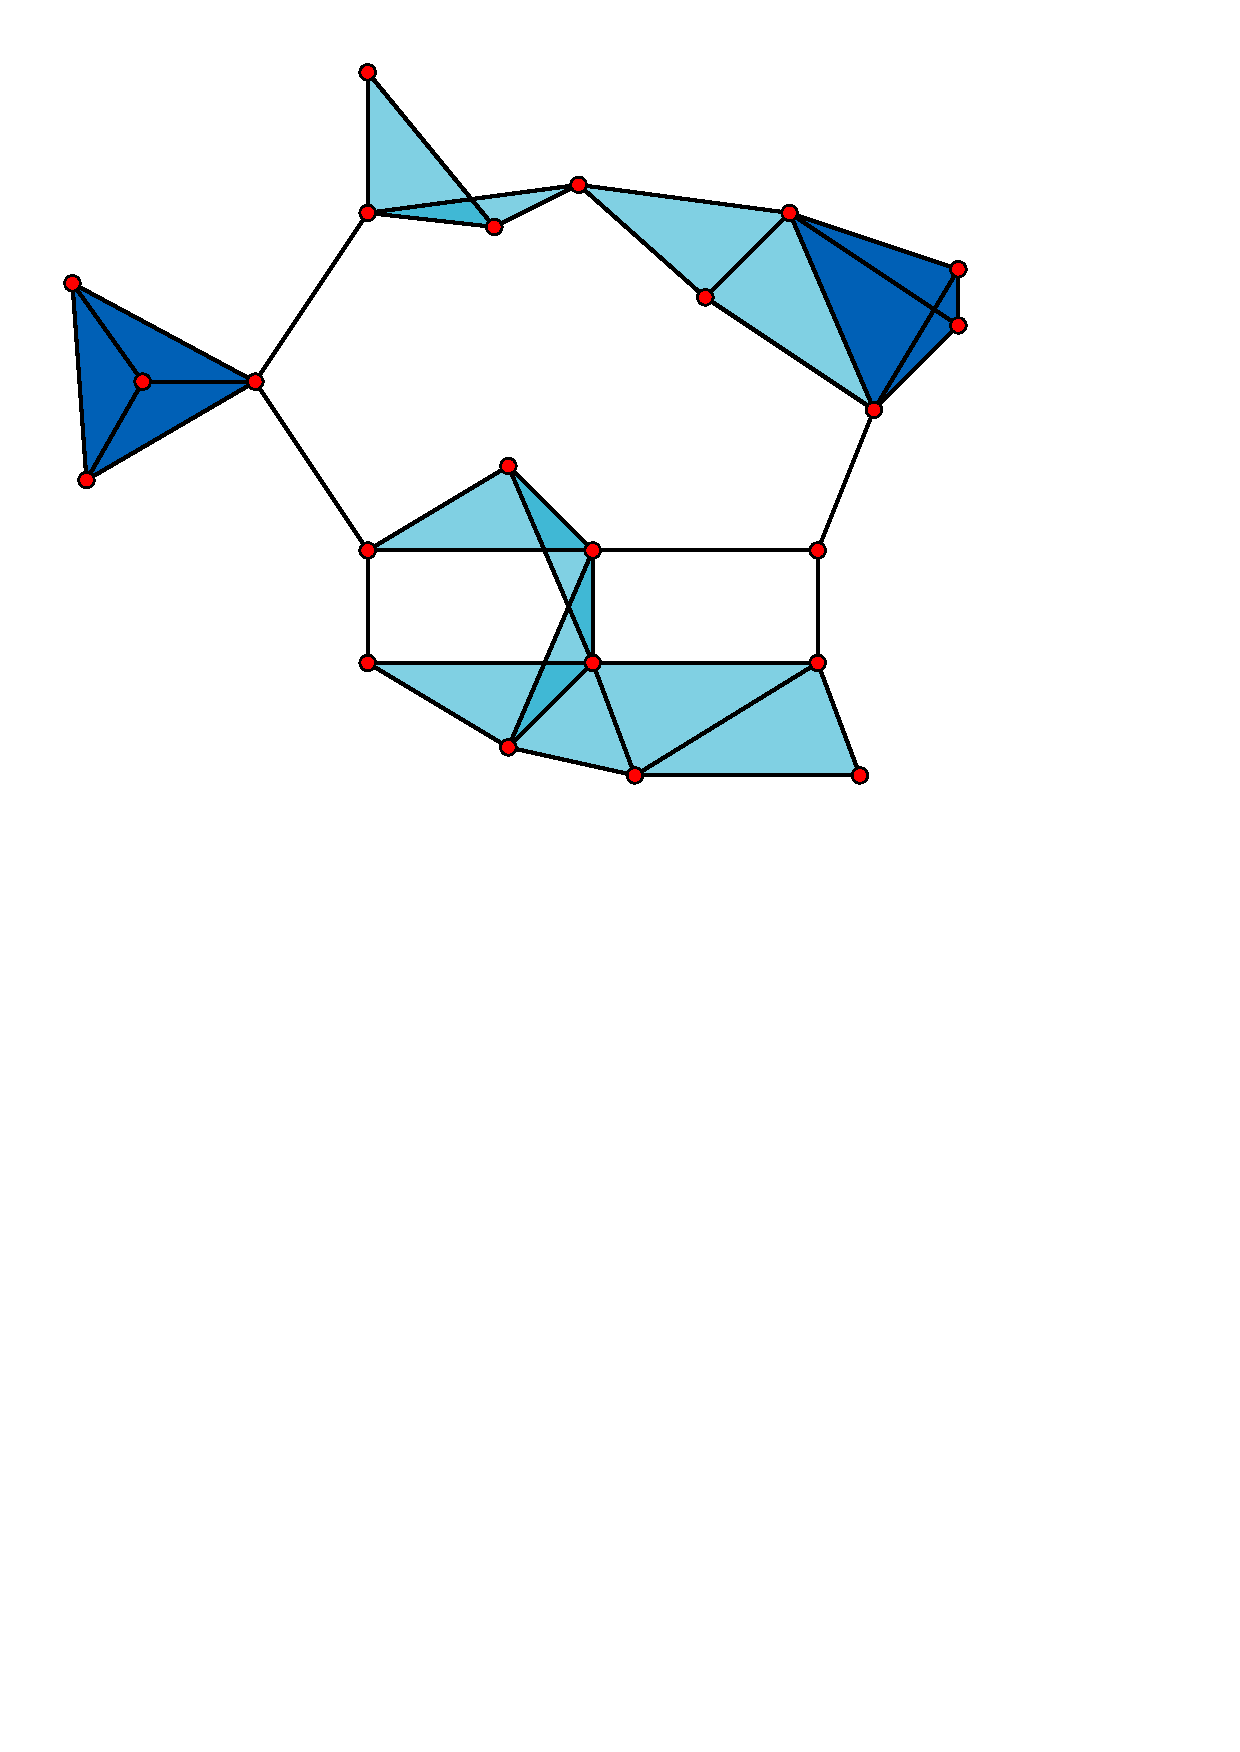
\includegraphics[width=0.8\textwidth]{clique}
\end{figure}
\end{minipage}

\begin{minipage}[c]{.7\textwidth}
Un'istanza del problema {\tsp} viene rappresentato dalle \(n\) città, da \(k\) e dalla matrice simmetrica \(d\) di distanze positive;
il più grande numero intero che appare nel problema viene determinato dal massimo fra \(n\), \(k\) e dal massimo valore contenuto nella matrice;
per memorizzare questo problema abbiamo bisogno di rappresentare la matrice in \(n^2\), e in più abbiamo bisogno di memorizzare il numero più grande presente nel problema.
\end{minipage}%
\begin{minipage}[c]{.3\textwidth}
\begin{figure}[H]\centering
	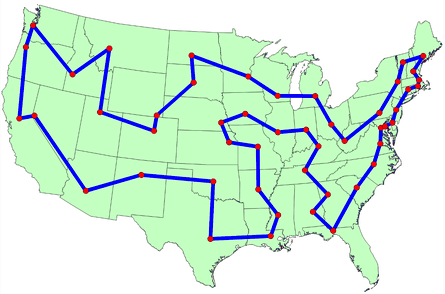
\includegraphics[width=0.8\textwidth]{tsp}
\end{figure}
\end{minipage}

\begin{definition}[problema fortemente \NP-completo]
Sia \(R_{\mathit{pol}}\) il problema \(R\) ristretto a quei dati d'ingresso per i quali il più grande valore da rappresentare è limitato superiormente da \(p(d)\), con \(p\) funzione polinomiale in \(d\) (\(d\) è la dimensione del mio input).
\(R\) è \alert{fortemente \NP-completo} se \(R_{\mathit{pol}}\) è \NP-completo.
\end{definition}

In altre parole, dato un problema che sappiamo essere \NP-completo, prendi il problema ristretto in cui metto dei limiti ai valori dei dati in input, questi limiti devono essere polinomiali nella dimensione del problema.
Se comunque il problema resto \NP-completo allora diremo che il problema è più che \NP-completo, è fortemente \NP-completo.

Se invece il problema non risulta più \NP-completo, e quindi finisce nello spazio {\PTIME}, allora si dice debolmente \NP-completo.

\begin{definition}[problema debolmente \NP-completo]
Se un problema \NP-completo non è fortemente \NP-completo, allora è \alert{debolmente \NP-completo}.
\end{definition}

\begin{observation}
Il problema cricca ({\cliqueProblem}), ad esempio, è fortemente \NP-completo, mentre quello della somma di sottoinsieme {\subSetSumProblem} non lo è.
\end{observation}

\subsection{Esempio di problema debolmente \NP-completo}

Sappiamo che il problema {\subSetSumProblem} è \NP-completo.

\subsubsection{Somma di sottoinsiemi (\subSetSumProblem)}

\paragraph{Definizione del problema}
Dati un vettore \(A\) contenente \(n\) interi positivi ed un intero positivo \(k\), \alert{esiste} un sottoinsieme \(S \subseteq \{1 \dots n\}\) tale che \(\sum_{i \in S} a[i] = k\)?

\begin{proof}[Dimostrazione. Somma di sottoinsieme è debolmente \NP-completo]
Possiamo imporre come limite che\newline \(\forall A[i] \leqslant k\) (valori più grandi di \(k\) vanno esclusi).
Se \(k = \Omicron(n^c)\), allora \(\texttt{\#} = \max\{n, k, a_1, \dots, a_n\} = \Omicron(n^c)\).
La soluzione basata su programmazione dinamica ha complessità \(\Omicron(nk) = \Omicron(n^{c+1})\), quindi in {\PTIME}.
Possiamo dedurne che {\subSetSumProblem} non è fortemente \NP-completo.
\end{proof}

\begin{note}
Il problema di {\subSetSumProblem} è debolmente \NP-completo: limitando le dimensioni dei dati in ingresso il problema diventa polinomiale.
\end{note}

\subsection{Algoritmi pseudo-polinomiali}

\begin{definition*}[Algoritmo pseudo-polinomiale]
Un algoritmo che risolve un certo problema \(R\), per qualsiasi dato \(I\) d'ingresso, in tempo \(p(\texttt{\#},d)\), con \(p\) funzione polinomiale in \texttt{\#} e \(d\), ha complessità \alert{pseudo-polinomiale}.
\end{definition*}

\begin{observation}
Gli algoritmi per {\subSetSumProblem} basati su programmazione dinamica e memoization sono pseudo-polinomiali.
\end{observation}

\begin{theorem*}
Nessun problema fortemente \NP-completo può essere risolto da un algoritmo pseudo-polinomiale, a meno che non sia \(\PTIME = \NP\).
\end{theorem*}

\subsection{Esempi di problemi fortemente \NP-completi}

\subsubsection{Cricca (\cliqueProblem)}

\paragraph{Definizione del problema}
Dati un grafo non orientato ed un intero \(k\), esiste un sottoinsieme di almeno \(k\) nodi tutti mutuamente adiacenti?

\begin{proof}[Dimostrazione. {\cliqueProblem} è fortemente \NP-completo]
Possiamo porre come limite \(k \leqslant n\), in quanto non ha senso chiedersi se esiste in un grafo con \(k\) nodi se esiste un sottografo con \(n\) nodi con \(n > k\), la risposta in quel caso è \False.
Quindi il valore massimo dei dati in ingresso \(\texttt{\#} = \max\{n,m,k\}\), in quanto \(k \leqslant n\) possiamo semplificare \(\texttt{\#} = \max\{n,m\}\).
La dimensione del problema è data da \(d = \Omicron(n + m + \log\texttt{\#})\), ma visto che sappiamo che \(\texttt{\#} = \max\{n,m\}\), allora possiamo semplificare e otteniamo \(d = \Omicron(n + m)\).
Quindi \(\texttt{\#} = \max\{n, m\}\) è limitato superiormente da \(\Omicron(n + m)\) qualunque siano i dati di ingresso.
Possiamo dedurne che il problema ristretto è identico a {\cliqueProblem}, che è \NP-completo.
\end{proof}

\begin{note}
Il problema {\cliqueProblem} è fortemente \NP-completo.
\end{note}

\subsubsection{Commesso viaggiatore (\tsp)}

\paragraph{Definizione del problema}
Date \(n\) città e una matrice simmetrica d di distanze positive, dove \(d[i][j]\) è la distanza fra \(i\) e \(j\), trovare un percorso che, partendo da una qualsiasi città, attraversi ogni città esattamente una volta e ritorni alla città di partenza, in modo che la distanza totale percorsa sia minima.

\begin{proof}[Dimostrazione per assurdo che {\tsp} è fortemente \NP-completo]
Per assurdo, supponiamo che {\tsp} sia debolmente \NP-completo.
Allora esiste una soluzione pseudo-polinomiale.
Usiamo questa soluzione per risolvere un problema \NP-completo in tempo polinomiale, il che è assurdo a meno che \(\PTIME = \NP\).
\end{proof}

Un problema se non ha valori numerici molto probabilmente risulta {\NP}-completo, mentre se li ha potrebbe essere o non essere debolmente {\NP}-completo.
Questo è un esempio di un problema che non lo è.

\begin{note}
Il problema {\tsp} è fortemente \NP-completo nonostante abbia valori numerici.
\end{note}

\subsubsection{Circuito hamiltoniano (\hamiltonianCircuit)}

\paragraph{Definizione del problema}
Dato un grafo non orientato \(G\), esiste un circuito che attraversi ogni nodo una e una sola volta?

Questo problema è fortemente collegato al problema del commesso viaggiatore, in quanto un tour del commesso viaggiatore è un circuito hamiltoniano.

\paragraph{Complessità}
Il problema {\hamiltonianCircuit} è \NP-completo.
\'{E} uno dei 21 problemi elencati nell'articolo di Karp.

\begin{proof}[Dimostriamo che {\tsp} è fortemente \NP-completo.]
Sia \(G = (V,E)\) un grafo non orientato.
Definiamo una matrice di distanze a partire da \(G\).
\[
	d[i][j] =
	\begin{dcases}
		1 & (i,j) \in E\\
		2 & (i,j) \not\in E\\
	\end{dcases}
\]

Il grafo \(G\) ha un circuito hamiltoniano se e solo se è possibile trovare un percorso da commesso viaggiatore di costo \(n\).

\paragraph{Simmetria fra {\tsp} e {\hamiltonianCircuit}}
Se esistesse un algoritmo pseudopolinomiale \(A\) per {\tsp}, {\hamiltonianCircuit} potrebbe essere risolto da \(A\) in tempo polinomiale.
La riduzione consiste nel prendere il circuito hamiltoniano dove il \(k\) cercato nel circuito hamiltoniano è pari alle \(n\) città.
\end{proof}

\begin{note}
Non sempre è semplice identificare immediatamente se un problema numerico risulti fortemente o debolmente \NP-completo.
\end{note}

\subsubsection{Partizione (\partition)}

\paragraph{Definizione del problema}
Dato un vettore \(A\) contenente \(n\) interi positivi, esiste un sottoinsieme \(S \subseteq \{1 \dots n\}\) tale che \(\sum_{i \in S} A[i] = \sum_{i \in S} A[i]\)?

\begin{figure}[H]
	\centering
	\begin{tikzpicture}
		\coordinate (t) at (.25,+.6);
		\foreach \num in {0,1,...,5}{
			\node[font=\tiny] at (t) {\num};
			\coordinate (t) at ($(t) + (0.6,0)$);
		}

		\coordinate (s) at (0,0);
		\foreach \num in {14,6,12,3,7,2}{
			% \node[draw, thick, rectangle, minimum size=0.5cm] at (s) {\num};
			\node[cell, minimum width = 0.6cm, minimum height = 0.6cm] at (s) {\num};
			\coordinate (s) at ($(s) + (0.6,0)$);
		}
	\end{tikzpicture}
\end{figure}

Ad esempio prendendo in considerazione questo vettore possiamo prendere gli insiemi \(\{14, 6, 2\}\) e \(\{12, 3, 7\}\).

\paragraph{Conclusioni}
\'{E} possibile ridurre il problema {\partition} a {\subSetSumProblem} scegliendo come valore \(k\) la metà di tutti i valori presenti:
\[
	k = \frac{\sum_{i=1}^{n} A[i]}{2} = \frac{44}{2} = 22
\]

\begin{note}
Il problema {\partition} è debolmente \NP-completo.
\end{note}

\subsubsection{3-Partizione (\treePartition)}

Dati \(3n\) interi \(\{a_1, \dots, a_{3n}\}\) esiste una partizione in \(n\) triple \(T_1, \dots, T_n\), tale che la somma dei tre elementi di ogni \(T_j\) sia la stessa, per \(1 \leqslant j \leqslant n\)?

\begin{note}
Il problema {\treePartition} è fortemente \NP-completo: non esiste un algoritmo pseudopolinomiale per risolverlo.
\end{note}

\section{Algoritmi di approssimazione}

Facciamo una piccola premessa.
I problemi più interessanti sono in forma di ottimizzazione.
Se il problema di decisione è \NP-completo, non sono noti algoritmi polinomiali per il problema di ottimizzazione.
Esistono però algoritmi polinomiali che trovano soluzioni ammissibili più o meno vicine a quella ottima.

\begin{definition*}[Algoritmi di approssimazione]
Se è possibile dimostrare un limite superiore/inferiore al rapporto fra la soluzione trovata e la soluzione ottima, allora tali algoritmi vengono detti \alert{algoritmi di approssimazione}.
\end{definition*}

\subsubsection*{Approssimazione}

\begin{definition*}[\(\alpha(n)-approssimazione\)]
Dato un problema di ottimizzazione con funzione costo non negativa \(c\), un algoritmo si dice di \alert{\(\alpha(n)\)-approssimazione} se fornisce una soluzione ammissibile \(x\) il cui costo \(c(x)\) non si discosta dal costo \(c(x^*)\) della soluzione ottima \(x^*\) per più di un fattore \(\alpha(n)\), per qualunque input di dimensione \(n\):
\begin{alignat*}{4}
	c(x^*) \leqslant c(x)           &\leqslant \alpha(n) c(x^*) &\quad& \alpha(n) > 1 \quad (\text{Minimizzazione})\\
	\alpha(n) c(x^*) \leqslant c(x) &\leqslant c(x^*)           &\quad& \alpha(n) < 1 \quad (\text{Massimizzazione})
\end{alignat*}
\end{definition*}

In altre parole se si sta cercando di minimizzare

\begin{observation}
\(\alpha(n)\) può essere una costante, valida per tutti gli \(n\).
\end{observation}

\begin{note}
Identificare un valore \(\alpha(n)\) e dimostrare che l'algoritmo lo rispetta è ciò che rende un buon algoritmo un algoritmo di approssimazione.
\end{note}

\subsection{Bin packing}

\paragraph{Definizione del problema}
Dati un vettore \(A\) contenente \(n\) interi positivi (i \alert{volumi} degli \alert{oggetti}) e un intero positivo \(k\) (la \alert{capacità} di una \alert{scatola}, tale che \(\forall i: A[i] \leqslant k\)), si vuole trovare una partizione di \(\{1, \dots, n\}\) nel minimo numero di sottoinsiemi disgiunti (\enquote{scatole}) tali che \(\sum_{i \in S} A[i] \leqslant k\) per ogni insieme \(S\) della partizione.

Dato il seguente vettore e un intero \(k = 8\) come risolvereste il problema?
\begin{figure}[H]
	\centering
	\begin{tikzpicture}
		\coordinate (t) at (.25,+.5);
		\foreach \num in {0,1,...,6}{
			\node[font=\tiny] at (t) {\num};
			\coordinate (t) at ($(t) + (0.5,0)$);
		}

		\coordinate (s) at (0,0);
		\foreach \num in {3,7,2,5,4,3,5}{
			\node[cell] at (s) {\num};
			\coordinate (s) at ($(s) + (0.5,0)$);
		}
	\end{tikzpicture}
\end{figure}

\subsubsection{Appoccio ingordo per bin packing}

\paragraph{Algoritmo first-fit}
Gli oggetti sono considerati in un ordine qualsiasi e ciascun oggetto è assegnato alla prima scatola che lo può contenere, tenuto conto di quanto spazio è stato occupato della stessa.

\begin{figure}[H]
	\centering
	\begin{tikzpicture}

		\coordinate (s) at (0,0);
		\foreach \num in {{3,2,3},7,5,4,5}{
			\node[cell, minimum width = 1.3cm] at (s) {\num};
			\coordinate (s) at ($(s) + (1.3,0)$);
		}
	\end{tikzpicture}
\end{figure}

In questo particolare caso si è comportato in maniera ottimale.

Sia \(N > 1\) il numero di scatole usare da {\firstFit} (se \(N=1\), l'algoritmo è ottimale).
Il numero minimo di scatole \(N^*\) è limitato da:
\[
	N^{*} \geqslant \ceil*{\frac{\sum_{i=1}^n A[i]}{k}} = \ceil*{\frac{29}{8}} = \ceil{3.625} = 4
\]
non possono esserci due scatole riempite meno della metà:
\[
	N < \frac{\sum_{i=1}^n A[i]}{k/2} = \frac{29}{8/2} = 7.250
\]
abbiamo quindi:
\[
	N < \frac{\sum_{i=1}^n A[i]}{k/2} = 2 \frac{\sum_{i=1}^n A[i]}{k} \leqslant 2N^* = \alpha(n) N^{*}
\]
che implica \(\alpha(n) = 2\).

\begin{note}
Nel peggiore dei casi l'algoritmo First-Fit utilizza il doppio delle scatole.
\end{note}

\paragraph{Algoritmo first-fit decreasing}
Se consideriamo gli oggetti in ordine non descrescente è possibile dimostrare un risultato migliore per l'algoritmo First-Fit.
\[
	N < \frac{17}{10} N^{*} + 2
\]
Nella variante \textsc{ffd} (First-fit decreasing): gli oggetti sono considerati in ordine non decrescente
\[
	N < \frac{11}{9} N^{*} + 4
\]
\begin{note}
Queste sono dimostrazioni di limiti superiori per il fattore \(\alpha(n)\), per casi particolari l'approssimazione può essere migliore.
\end{note}

\subsection{Commesso viaggiatore con disuguaglianze triangolari ({\deltaTsp})}

\paragraph{Definizione del problema}
Siano date \(n\) città e le distanze (positive) \(d[i][j]\) tra esse, \alert{tale per cui vale la regola delle diseguaglianze triangolari}:
\[
	d[i][j] \leqslant d[i][k] + d[k][j] \quad \forall i,j,k: \quad 1 \leqslant i,j,k \leqslant n
\]
Trovare un percorso che, partendo da una qualsiasi città, attraversi ogni città esattamente una volte e ritorni alla città di partenza, in modo che la distanza complessiva percorsa sia minima.

\begin{figure}[H]
	\begin{subfigure}[t]{.5\linewidth}\centering
		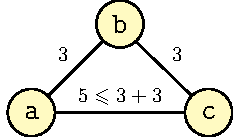
\includegraphics[page=1]{triangle-inequality}
		\caption{con diseguaglianza triangolare}
	\end{subfigure}%
	\begin{subfigure}[t]{.5\linewidth}\centering
		\includegraphics[page=2]{triangle-inequality}
		\caption{senza diseguaglianza triangolare}
	\end{subfigure}
\end{figure}

\begin{note}
{\deltaTsp} è \NP-completo.
\end{note}

\begin{proof}[Dimostriamo che {\hamiltonianCircuit} \(\leqslant_p\) {\deltaTsp}]
Sia \(G = (V, E)\) un grafo non orientato. Definiamo una matrice delle distanze a partire da \(G\)
\[
	d[i][j] =
	\begin{dcases}
		1 & (i,j) \in E\\
		2 & (i,j) \not\in E\\
	\end{dcases}
\]
Abbiamo applicato la stessa riduzione che avevamo applicato per il problema {\tsp}.
Il grafo \(G\) ha un circuito hamiltoniano se e solo se è possibile trovare un percorso da commesso viaggiatore lungo \(n\).
Valgono le diseguaglianze triangolari:
\[
	d[i][j] \leqslant 2 \leqslant d[i][k] + d[k][j]\qedhere
\]
Questo particolare grafo gode di disuguaglianza triangolare perché \(d[i][j]\) può avere valore massimo 2, mentre \(d[i][k]\) e \(d[k][j]\) hanno come valori minimi 1.
\end{proof}

\begin{note}
Se esistesse una soluzione polinomiale (in {\PTIME}) per {\deltaTsp}, allora esisterebbe anche una soluzione per {\hamiltonianCircuit} cosa che non riteniamo possibile.
\end{note}

\subsubsection{Commesso viaggiatore come circuito hamiltoniano pesato}

Interpretiamo {\deltaTsp} come il problema di trovare un circuito hamiltoniano di peso minimo su un grafo completo.

\begin{figure}[H]\centering
	\hfill
	\begin{subfigure}[c]{.22\linewidth}\centering
		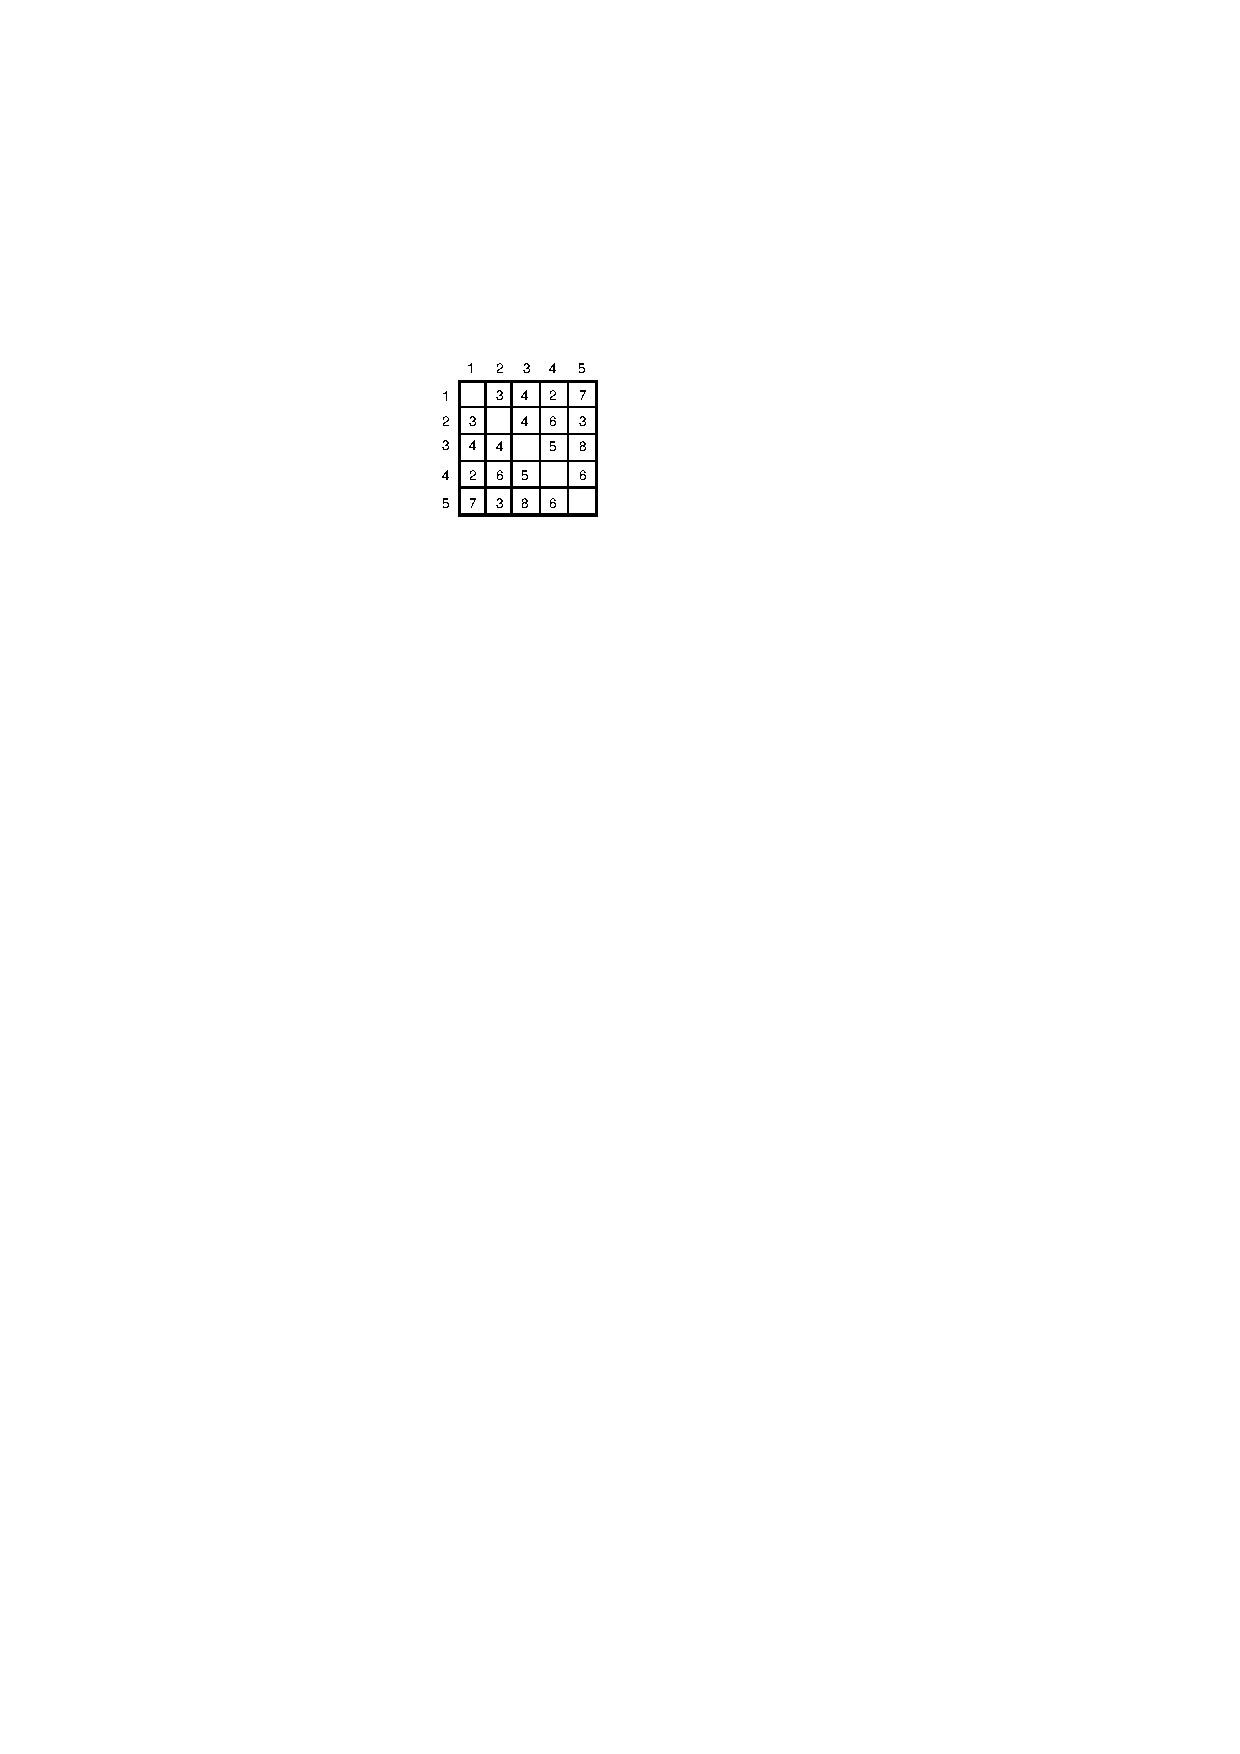
\includegraphics{tsp-greedy}
	\end{subfigure}%
	\hfill
	\begin{subfigure}[c]{.22\linewidth}\centering
		\includegraphics[page=9, width=\linewidth]{tsp-pentagon}
	\end{subfigure}%
	\hfill
	\begin{subfigure}[c]{.22\linewidth}\centering
		\includegraphics[page=5, width=\linewidth]{tsp-local}
	\end{subfigure}%
	\hfill\null
	\caption{Il costo totale risulta 21. Il costo totale risulta 19.}
\end{figure}

\subsubsection{Algoritmo di approssimazione per {\deltaTsp}}

Se si considera un circuito hamiltoniano e si cancella un suo arco, si ottiene un albero di copertura.

\begin{figure}[H]\centering
	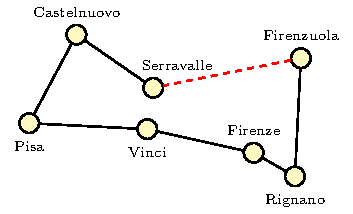
\includegraphics[page=1, width=0.5\linewidth]{toscana}
\end{figure}

Che relazione hanno gli alberi di copertura con i circuiti hamiltoniani?

\begin{theorem*}
Qualunque circuito hamiltoniano \(\pi\), ha costo \(c(\pi)\) superiore al costo \(\mathit{mst}\) di albero di copertura di peso minimo, ovvero \(\mathit{mst} < c(\pi)\).
\end{theorem*}

\begin{proof}[Dimostrazione per assurdo.]
Supponiamo che esista un circuito hamiltoniano \(\pi\) di costo \(c(\pi) \leqslant \mathit{mst}\).
Togliamo un arco, otteniamo un albero di copertura con peso inferiore \(\mathit{mst}' < c(\pi) \leqslant \mathit{mst}\).
Contraddizione, visto che \(\mathit{mst}\) è il costo minimo fra tutti gli alberi di copertura.
\end{proof}

\subsubsection{Algoritmo per {\deltaTsp}}

Si individua un minimo albero di copertura di peso \(\mathit{mst}\) e se ne percorrono gli archi due volte, prima in un senso e poi nell'altro.
In questo modo, si visita ogni città almeno una volta.
La distanza complessiva di tale circuito è uguale a \(2 \cdot mst\).
Ma non è un circuito hamiltoniano!

\begin{figure}[H]\centering
	\begin{subfigure}[t]{.5\linewidth}\centering
		\includegraphics[page=2, width=.8\linewidth]{toscana}
	\end{subfigure}%
	\begin{subfigure}[t]{.5\linewidth}\centering
		\includegraphics[page=3, width=.8\linewidth]{toscana}
	\end{subfigure}
\end{figure}

Si evita di passare per città già visitate, saltandole.
Per la diseguaglianza triangolare, il costo \(c(\pi)\) del circuito così ottenuto è inferiore o uguale a \(2 \cdot \mathit{mst}\).
Concludendo, \(c(\pi) \leqslant 2 \cdot \mathit{mst} < 2 \cdot 2 \cdot c(\pi^*)\) implica che \(\alpha(n) = 2\), dove \(c(\pi^*)\) è il costo del circuito hamiltoniano ottimo.

\begin{figure}[H]\centering
	\begin{subfigure}[t]{.5\linewidth}\centering
		\includegraphics[page=4, width=.8\linewidth]{toscana}
	\end{subfigure}%
	\begin{subfigure}[t]{.5\linewidth}\centering
		\includegraphics[page=5, width=.8\linewidth]{toscana}
	\end{subfigure}
\end{figure}

\subsubsection{Discussione sulla complessità dell'algoritmo per {\deltaTsp}}

La complessità dell'algoritmo è pari a \(\Omicron(n^2 \log n)\).
I fattori che contribuiscono sono:
\begin{itemize}
	\item \(\Omicron(n^2 \log n)\) per l'algoritmo di Kruskal;
	\item \(\Omicron(n)\) per la visita in profondità del \(\mathit{mst}\) con \(2n\) archi.
\end{itemize}
Tuttavia esistono grafi \enquote{perversi} per cui il fattore di approssimazione tende al valore 2.
L'algoritmo di Christofides (1976) ha un fattore di approssimazione di 3/2, il migliore risultato al momento.

\subsubsection{Non approssimabilità di {\tsp}}

Abbiamo visto che {\deltaTsp} può essere approssimato.
Non esiste alcun algoritmo di \(\alpha(n)\)-approssimazione per {\tsp} tale che \(c(x') \leqslant sc(x^*)\), con \(s \geqslant 2\) intero positivo, a meno che non sia \(\PTIME = \NP\).

\begin{note}
\(\Delta-tsp\) è un problema approssimabile, ma il problema generale non lo è.
\end{note}

\section{Algoritmi euristici}

Quando si è presi dalla disperazione a causa della enorme difficoltà di un problema di ottimizzazione {\NP}-hard, si può ricorrere ad algoritmi \enquote{euristici} che forniscono una soluzione ammissibile.
La soluzione fornita non è necessariamente ottima, né necessariamente approssimata.
Talvolta non si riesce a dimostrare che non sia possibile fare meglio di così.

Le tecniche che è possibile utilizzare in questi casi sono l'approccio ingordo e la ricerca locale.

\newpage
\subsection{Approccio ingordo per {\tsp}}

\subsubsection{Algoritmo \enquote{Shortest edges first}}

Ordiniamo gli archi per pesi non decrescenti e aggiungiamo archi alla soluzione seguendo questo ordine finché non sono stati aggiunti \(n-1\) archi, dove \(n\) è il numero di nodi.

Per poter aggiungere un arco, occorre verificare che
\begin{itemize}
	\item per ciascuno dei suoi nodi non siano stati già scelti due archi;
	\item che non si formino circuiti (questo lo si fa tramite l'utilizzo della struttura dati {\mfSet}).
\end{itemize}
A questo punto, si è trovata una catena Hamiltoniana (un percorso che tocca tutti i nodi ma che non tocca il nodo di partenza).
Si chiude il circuito aggiungendo l'arco tra i due nodi estremi della catena.

\begin{figure}[H]\centering
	\begin{subfigure}{.25\linewidth}\centering
		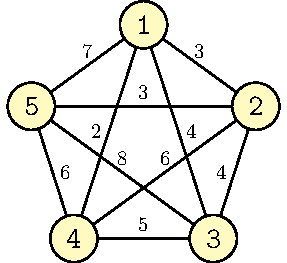
\includegraphics[page=1, width=\linewidth]{tsp-pentagon}
	\end{subfigure}%
	\begin{subfigure}{.25\linewidth}\centering
		\includegraphics[page=2, width=\linewidth]{tsp-pentagon}
	\end{subfigure}%
	\begin{subfigure}{.25\linewidth}\centering
		\includegraphics[page=3, width=\linewidth]{tsp-pentagon}
	\end{subfigure}%
	\begin{subfigure}{.25\linewidth}\centering
		\includegraphics[page=4, width=\linewidth]{tsp-pentagon}
	\end{subfigure}

	\vspace{10pt}

	\begin{subfigure}{.25\linewidth}\centering
		\includegraphics[page=5, width=\linewidth]{tsp-pentagon}
	\end{subfigure}%
	\begin{subfigure}{.25\linewidth}\centering
		\includegraphics[page=6, width=\linewidth]{tsp-pentagon}
	\end{subfigure}%
	\begin{subfigure}{.25\linewidth}\centering
		\includegraphics[page=7, width=\linewidth]{tsp-pentagon}
	\end{subfigure}%
	\begin{subfigure}{.25\linewidth}\centering
		\includegraphics[page=8, width=\linewidth]{tsp-pentagon}
	\end{subfigure}%

	\caption[Applicazione dell'algoritmo ingordo \enquote{Shortest edges first} per {\tsp}]{Applicazione dell'algoritmo \enquote{Shortest edges first}. Questo algoritmo parte dagli archi, scegliendo sempre l'arco con peso minore. Non è possibile aggiungere i nodi con peso 4 perché i nodi che toccano hanno già due archi selezionati. Il costo totale del percorso con questo algoritmo risulta 21.}
\end{figure}

\begin{algorithm}[H]
	\caption{Risoluzione del commesso viaggiatore con algoritmo ingordo}
	%&../preamble

% arara: pdflatex: { synctex: no }
% arara: latexmk: { clean: partial }
\ifstandalone
\begin{document}
\begin{algorithm}[H]
\fi

\prototype{\Set \greedyTsp{\Graph \(G\)}}{

	\BlankLine
	\tcp{creazione strutture dati}
	\Set \(result \Assign  \setConstructor\)\;
	\mfSet \(M \Assign  \mfConstructor{G.\setSize}\)\;
	\tcp{archi in ingresso ad un nodo}
	\Array{\Int} \(edges\) \Assign \new \Array{\Int}[1][G.\setSize] = \{ 0 \} \tcp{no.\ archi della catena}

	\BlankLine
	\(A\) \Assign \{ ordina gli archi per peso decrescente \}

	\BlankLine
	\tcp{per ogni arco che appartiene all'insieme degli archi}
	\ForEach{\((u,v) \in A\)}{
		\tcp{se gli archi entranti in entrambi i nodi sono minori di 2 e non si è formato un circuito}
		\If{\(edges[u] < 2\) \And \(edges[v] < 2\) \And \(M.\mfFind{u} \Neq M.\mfFind{v}\)}{

			\BlankLine
			\tcp{prendo nota dell'arco inserito}
			\(S.\setInsert{\((u,v)\)}\)\;

			\BlankLine
			\tcp{aggiorno il no.\ di lati entranti nei due nodi}
			\(\Increment{edges[u]}\)\;
			\(\Increment{edges[v]}\)\;

			\BlankLine
			\tcp{li considero come un unico nodo}
			\(M.\mfMerge{u,v}\)\;
		}
	}

	\BlankLine
	\tcp{chiudo il circuito}
	\Int \(u \Assign  1\)\;
	\lWhile{\(edges[1] \Neq 1\)}{
		\(\Increment{u}\)
	}

	\BlankLine
	\Int \(v \Assign  u + 1\)\;
	\lWhile{\Not \(edges[v] \Neq 1\)}{
		\(\Increment{v}\)
	}

	\BlankLine
	\tcp{chiusura del circuito hamiltoniano}
	\(S.\setInsert{\((u,v)\)}\)

	\BlankLine
	\tcp{restituisco l'insieme che archi che costituisce il percorso}
	\Return \(S\)\;
}

\ifstandalone
\end{algorithm}
\end{document}
\fi

\end{algorithm}

\newpage
\subsubsection{Algoritmo \enquote{Nearest Neighbor}}

Possiamo usare un approccio diverso.
Si parte da una città, si seleziona come prossima città quella più vicina (con distanza più bassa) e si va avanti così, evitando città già visitate.
Quando si sono visitate tutte le città, si torna alla città di partenza.

Così facendo possiamo lavorare direttamente sulla matrice, senza usare strutture di appoggio (come il grafo dell'esempio precedente).

\begin{figure}[H]\centering
	\begin{subfigure}{.25\linewidth}\centering
		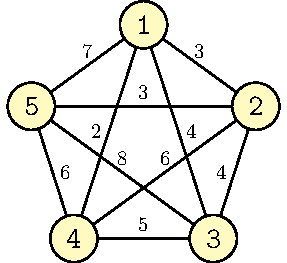
\includegraphics[page=1, width=\linewidth]{tsp-nn}
	\end{subfigure}%
	\begin{subfigure}{.25\linewidth}\centering
		\includegraphics[page=2, width=\linewidth]{tsp-nn}
	\end{subfigure}%
	\begin{subfigure}{.25\linewidth}\centering
		\includegraphics[page=3, width=\linewidth]{tsp-nn}
	\end{subfigure}%
	\begin{subfigure}{.25\linewidth}\centering
		\includegraphics[page=4, width=\linewidth]{tsp-nn}
	\end{subfigure}%

	\vspace{10pt}

	\begin{subfigure}{.25\linewidth}\centering
		\includegraphics[page=5, width=\linewidth]{tsp-nn}
	\end{subfigure}%
	\begin{subfigure}{.25\linewidth}\centering
		\includegraphics[page=6, width=\linewidth]{tsp-nn}
	\end{subfigure}%
	\begin{subfigure}{.25\linewidth}\centering
		\includegraphics[page=7, width=\linewidth]{tsp-nn}
	\end{subfigure}%
	\begin{subfigure}{.25\linewidth}\centering
		\includegraphics[page=8, width=\linewidth]{tsp-nn}
	\end{subfigure}%

	\caption[Applicazione dell'algoritmo ingordo \enquote{Nearest Neighbor} per {\tsp}]{Applicazione dell'algoritmo \enquote{Nearest Neighbor}. Il costo totale del percorso con questo algoritmo risulta 21, come nel caso precedente.}
\end{figure}

\subsubsection{Discussione sulla complessità dell'approccio ingordo per {\tsp}}

Il costo computazionale dell'algoritmo \enquote{Shortest edges first} ha un costo computazionale di \(\Omicron(n^2 \log n)\), dove \(\log n\) è dovuto all'ordinamento degli archi; mentre l'algoritmo \enquote{Nearest Neighbor} ha un costo di \(\Omicron(n^2)\).

La soluzione così ottenuta si può utilizzare può essere migliorata ancora tramite ricerca locale e può essere usata come base di partenza per un algoritmo branch-\&-bound.

\subsection{Approccio ricerca locale per {\tsp}}

\subsubsection{Algoritmo di ricerca locale}

Sia \(\pi\) un circuito Hamiltoniano del grafo completo derivante dal problema {\tsp}.
Si consideri il seguente intorno:
\(I_2(\pi) =\) \{\(\pi'\): \(\pi'\) è ottenuto da \(\pi\) cancellando due archi non consecutivi del circuito e sostituendoli con due archi esterni al circuito\}

\begin{note}
La cardinalità di \(I_(\pi)\) è \(\abs{I_(\pi)} = \frac{n(n-1)}{2}-n\), in quanto ci sono \(\frac{n(n-1)}{2}\) coppie di archi del circuito e \(n\) di esse sono consecutive.

Una volta spezzato il circuito, esiste un solo modo per riconnetterlo.
\end{note}

\begin{figure}[H]\centering
	\begin{subfigure}[c]{.4\linewidth}\centering
		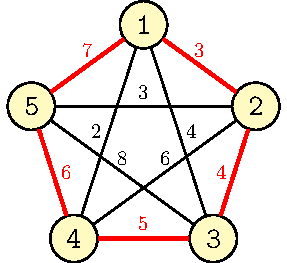
\includegraphics[page=1, width=.5\linewidth]{tsp-local}\hfill
		\includegraphics[page=2, width=.5\linewidth]{tsp-local}
		\caption{Costo: 25.}
	\end{subfigure}%
	\begin{subfigure}[c]{.4\linewidth}\centering
		\includegraphics[page=3, width=.5\linewidth]{tsp-local}\hfill
		\includegraphics[page=4, width=.5\linewidth]{tsp-local}
		\caption{Costo: 23.}
	\end{subfigure}%
	\begin{subfigure}[c]{.20\linewidth}\centering
		\includegraphics[page=5, width=\linewidth]{tsp-local}
		\caption{Costo: 19.}
	\end{subfigure}%
	\caption[Applicazione dell'algoritmo di ricerca locale per {\tsp}]{Il costo totale del percorso con questo algoritmo risulta 19, che risulta ottimo.}
\end{figure}

\subsubsection{Discussione sulla complessità dell'approccio di ricerca locale per {\tsp}}

Il costo per esaminare \(I_2(\pi)\) è \(\Omicron(n^2)\).

\section{Algoritmi branch\&bound}

A differenza delle tecniche di approssimazione che rinunciavano alla formalità nella risoluzione di un problema pur di ottenere un algoritmo polinomiale, per risolvere un problema di ottimizzazione \NP-arduo, si può modificare la procedura \enumeration, vista nel capitolo sul \foreign{backtracking}, in modo da \enquote{potare} certe sequenze di scelte che di rivelino incapaci di generare la soluzione ottima.

Facciamo una serie di assunzioni senza perdere troppa generalità:
\begin{itemize}
	\item problema di ottimizzazione;
	\item ogni sequenza di scelte abbia costo non negativo;
	\item ogni scelta, aggiunta alle scelte già effettuate, non faccia diminuire il costo della soluzione parziale così ottenuta.
\end{itemize}

\begin{algorithm}[H]
	\caption{Ripasso della procedura di enumerazione delle soluzioni}
	%&../preamble

% arara: pdflatex: { synctex: no }
% arara: latexmk: { clean: partial }
\ifstandalone
\begin{document}
\begin{algorithm}[H]
\fi

\prototype{\Bool \enumeration{\datiProblema, \Item{} \(S\), \Int i, \datiParziali}}{
	\params{S}[vettore contenente le soluzioni parziali \(S[1][i]\)]
	\params{i}[indice della scelta corrente]

	\BlankLine
	\BlankLine
	\uIf{\isAdmissible{\datiProblema, \(S\), \(i\), \datiParziali}}{
		\tcp{è una soluzione ammissibile}
		\If{\processSolution{\datiProblema, \(S\), \(i\), \datiParziali}}{
			\tcp{vogliamo bloccare l'esecuzione alla prima soluzione trovata}
			\Return \True \tcp{trovata soluzione, restituisco \True}
		}
	}
	\uElseIf{\reject{\datiProblema, \(S\), \(i\), \datiParziali}}{

		\BlankLine
		\Return \False \tcp{impossibile trovare soluzioni, restituisco \False}
	}
	\Else{
		\Set \(C\) \Assign \getChoices{\datiProblema, \(S\), \(i\), \datiParziali} \tcp{l'insieme delle scelte possibili}

		\BlankLine
		\ForEach(\tcp*[h]{per ogni possibile scelta fra quelle possibili}){\(c \in C\)}{
			\(S[i]\) \Assign \(c\) \tcp{memorizzo la scelta parziale}

			\BlankLine
			\tcp{richiamo ricorsivamente l'algoritmo effettuando la scelta successiva}
			\If{\enumeration{\datiProblema, \(S\), \(i+1\), \datiParziali}}{
				\Return \True \tcp{trovata soluzione, restituisco \True}
			}
		}
	}
	\Return \False \tcp{nessuna soluzione, restituisco \False}
}

\ifstandalone
\end{algorithm}
\end{document}
\fi

\end{algorithm}

Cerchiamo i limiti (superiore ed inferiore) della soluzione minima.

\subsubsection{Limite superiore}

Durante l'enumerazione, si mantengono informazioni sulla miglior soluzione ammissibile (\(minSol\)) ed il suo costo (\(minCost\)).
\(minCost\) costituisce un limite superiore (\foreign{upper bound}) per il costo della soluzione minima.

\subsubsection{Limite inferiore}

Si supponga di avere a disposizione una opportuna funziona \enquote{lower bound} {\lowerBound{\(\angleled{dati\ problema}\), S, i, \(\angleled{dati\ parziali}\)}}, che dipenda dalla sequenza di scelte fatte in precedenza \(S[1 \dots i]\), e che garantisca che tutte le soluzioni ammissibili generabili facendo nuove scelte abbiano costo \(\geqslant \lowerBound\).

\begin{figure}[H]
	\centering
	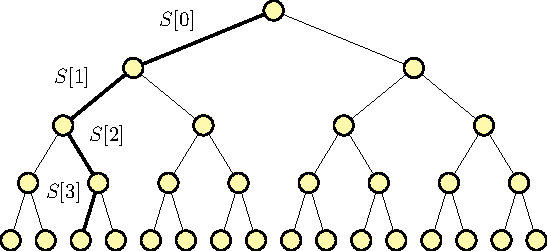
\includegraphics{branchAndBound-1}
	\caption[Esempio di potatura nell'albero di scelte per un algoritmo branch-\&-bound]{Se \textsf{lb}(\(S\),\(i\)) è maggiore o uguale a \(minCost\), allora si può evitare di generare ed esplorare il sottoalbero delle scelte radicato in tal nodo, effettuando così una \textbf{potatura}.}
\end{figure}

Questo metodo non migliora la complessità (superpolinomiale) della procedura \enumeration, ma nella pratica ne abbassa di molto il tempo di esecuzione.
Tutto dipende dalla funzione \lowerBound (che dobbiamo definire noi), che deve approssimare il più possibile il costo della soluzione ottima.
Il limite superiore è dato dal \(minCost\).

\begin{algorithm}[H]
	\caption{Somma di sottoinsiemi}
	%&../preamble

% arara: pdflatex: { synctex: no }
% arara: latexmk: { clean: partial }
\ifstandalone
\begin{document}
\begin{algorithm}[H]
\fi

\prototype{\branchAndBound{\datiProblema, \Item{} \(S\), \Int \(i\), \datiParziali}}{
	\Set \(C \Assign \getChoices{\datiProblema, n, i, \datiParziali}\) \Comment*[l]{determina l'insieme in funzione delle scelte precedenti \(S[1 \dots i-1]\)}

	\BlankLine
	\tcp{esamino ogni scelta}
	\ForEach{\(c \in C\)}{

		\BlankLine
		\(S[i] \Assign c\) \tcp{effettuo la scelta \(i\)-esima}

		\BlankLine
		\tcp{calcolo il lower bound in base alle scelte fasse in precedenza}
		\Int \(lb \Assign \lowerBound{\datiProblema, S, i, \datiParziali}\)\;

		\BlankLine
		\If(\tcp*[h]{se il limite inferiore non eccede il costo minimo}){\(lb < minCost\)}{

			\BlankLine
			\uIf(\tcp*[h]{posso ancora effettuare delle scelte}){\(i < n\)}{

				\BlankLine
				\tcp{faccio ricorsivamente le scelte successive}
				\branchAndBound{\datiProblema, S, \(i+1\), \datiParziali}
				\BlankLine

			}
			\Else{
				\tcp{ho effettuato tutte le scelte possibili (\(i \Equal n\))}

				\BlankLine
				\tcp{se il costo della soluzione trovata è minore del costo della soluzione parziale}
				\If{\(\cost(S,i) < minCost\)}{
					\tcp{allora la soluzione trovata è migliore del minimo parziale}

					\BlankLine
					\(minSol \Assign S\) \Comment*[l]{aggiorno la soluzione minima parziale}
					\(minCost \Assign \cost(S,i)\)  \Comment*[l]{aggiorno il costo minimo parziale}
				}
			}
		}

	}
}

\ifstandalone
\end{algorithm}
\end{document}
\fi

\end{algorithm}

\subsection{Approccio branch-\&-Bound per {\tsp}}

Sia \(n\) il numero delle città, e \(d[h][k]\) la distanza, intera e non negativa, fra le città \(h\) e \(k\).
Al passo \(i\)-esimo sono state fatte le scelte \(S[1 \dots i]\) prese dall'insieme \(\{1, \dots, n\}\).
Un percorso ammissible che \enquote{espande} \(S[1 \dots i]\) deve
\begin{enumerate}[label=\arabic*)]
	\item attraversare le città \(S[1 \dots i]\);
	\item passare da \(S[i]\) ad una qualsiasi delle rimanenti \(n-1\) città;
	\item attraversare queste ultime città in un ordine qualsiasi;
	\item da una di queste ritornare a \(S[1]\).
\end{enumerate}

La distanza percorsa finora è \(\cost[i]\), ossia il costo che ho sostenuto per fare i primi \(i\) passi.
\[
	\cost[i] =
	\begin{dcases}
		0                               & i = 1\\
		\cost[i-1] + d[ S[i-1] ][ S[i] ] & i > 1\\
	\end{dcases}
\]
Viene calcolata ricorsivamente dalla sommando il costo sostenuto per arrivare alla città precedente (\(\cost[i-1]\)) e la distanza intercorsa fra la città precedente e quella attuale.

\begin{minipage}[c]{.45\textwidth}
Il limite inferiore (\foreign{lower bound}) della distanza per "uscire" da \(S[i]\) (ha un costo di \(O(n)\)):
\[
	\out  = \min_{h \notin S} \{ d[S[i], h] \}
\]
\end{minipage}\hfill
\begin{minipage}[c]{.45\textwidth}
Il limite inferiore (\foreign{lower bound}) della distanza per tornare a \(S[1]\) (ha un costo di \(O(n)\)):
\[
	\back = \min_{h \notin S} \{ d[h, S[1]] \}
\]
\end{minipage}

% TODO produrre grafica esplicativa per le formule

Il limite inferiore della distanza percorsa per attraversare una qualsiasi di queste ultime città \(h\) delle \(n - i\) città, provenendo da (e dirigendosi verso) una città non compresa in \(S[2\dots n]\) (ha un costo di \(\Omicron(n^3)\)).
\[
	\forall h \not\in S: \transfer = \min_{p,q \not\in S[2\dots i-1]}\{d[p, h] + d[h, q] \colon h \Neq p \Neq q \}
\]

Se posso effettuare ancora delle scelte (\(i < n\)), è possibile calcolare un possibile limite inferiore \(\lowerBound{d, S, i}\) calcolando la somma:
\begin{itemize}
	\item del costo \(cost[i]\) per arrivare al nodo \(S[i]\), già speso;
	\item metà del costo ottenuto sommando:
	\begin{itemize}
		\item il limite inferiore \(out\) del costo per andare dal nodo \(S[i]\) ad un qualunque altro nodo;
		\item il limite inferiore per attraversare i nodi non contenuti in \(S\);
		\item il limite inferiore \(\back\) del costo per tornare al nodo \(S[i]\) da un qualunque altro nodo.
	\end{itemize}
\end{itemize}
\[
	\lowerBound(d,S,i) = cost[i] + \ceil*{\frac{\out + \sum_{h \not\in S} \transfer[h] + \back}{2}}
\]

\begin{algorithm}[H]
	\caption{Appoccio branch\&bound al problema del commesso viaggiatore}
	%&../preamble

% arara: pdflatex: { synctex: no }
% arara: latexmk: { clean: partial }
\ifstandalone
\begin{document}
\begin{algorithm}[H]
\fi

\prototype{\bbTsp{\Array{} \(S\), \Int \(\cost\), \Set \(R\), \Int \(n\), \Int \(i\)}}{

	\BlankLine
	\Set \(\choices\) \Assign \copyFunction{\(R\)}\;

	\ForEach{\(c \in \choices\)}{

		\BlankLine
		\(S[i] \Assign c\) \tcp{memorizza la scelta}

		\BlankLine
		\tcp{MECCANISMO PER GENERARE LE PERMUTAZIONI}
		\(R.\setRemove{c}\) \tcp{rimuovi la scelta nell'insieme delle scelte possibili}

		\BlankLine
		\tcp{MECCANISMO DI VALUTAZIONE}
		\eIf{\(i < n\)}{

			\BlankLine
			\{ calcola \(\out\), \(\back\), \(\transfer[h]\) per ogni \(h \in R \Leftrightarrow h \not\in S[1\dots i]\) \}

			\BlankLine
			\Int \(\lb\) \Assign \(\ceil*{\frac{\out + \sum_{h \not\in S} \transfer[h] + \back}{2}}\)

			\BlankLine
			\If{\(\lb < \minCost\)}{
				\bbTsp{\(S\), \(\cost + d[S[i-1]][S[i]]\), \(R\), \(i+1\)}\;
			}
		}{

			\BlankLine
			\(\lb\) \Assign \(\cost + d[S[i]][S[1]]\) \tcp{aggiorna il limite inferiore}

			\BlankLine
			\If(\tcp*[h]{se abbiamo trovato una soluzione migliore}){\(\lb < \minCost\)}{

				\BlankLine
				\(minSol\) \Assign \copyFunction{\(S\)} \tcp{aggiorna la soluzione ottimale}
				\(minCost\) \Assign \(\lb\) \tcp{aggiorna il costo minimo}
			}
		}

		\BlankLine
		\(R.\setInsert{c}\) \tcp{reinserisco la scelta nell'insieme delle scelte possibili}
	}
}

\ifstandalone
\end{algorithm}
\end{document}
\fi

\end{algorithm}

\subsubsection{Precisazione sull'algoritmo}

\(\minCost\) è una variabile globale.
Invece di inizializzarla a \(+\infty\), possiamo scegliere una permutazione a caso (un cammino qualunque), in questo modo abbiamo già una stima iniziale.
Ad esempio la permutazione 1-2-3-4-5 ha un costo pari a \(21\).
Per evitare che lo stesso circuito sia generato più volte, si parte da un nodo fissato (ad esempio 1).

\begin{figure}[H]
	\begin{subfigure}{.25\linewidth}\centering
		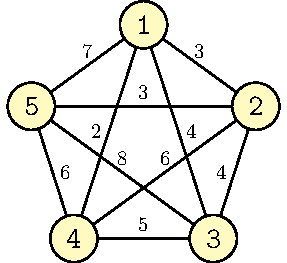
\includegraphics[width=.8\textwidth, page=1]{tsp-pentagon}
	\end{subfigure}%
	\begin{subfigure}{.75\linewidth}\centering
		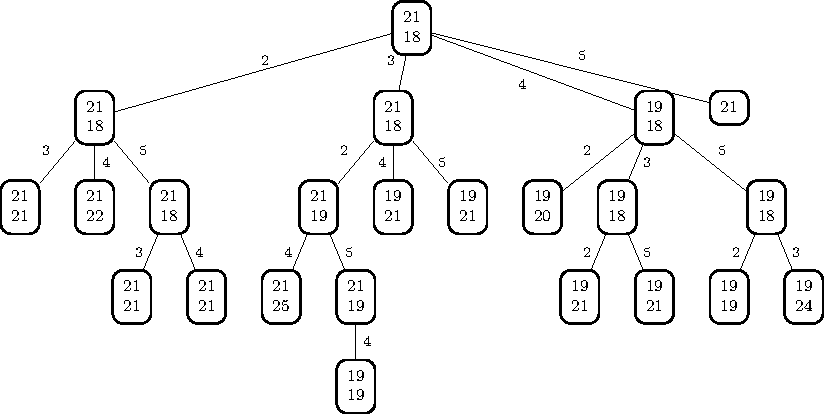
\includegraphics[width=\textwidth]{branchAndBound-2}
	\end{subfigure}
	\caption[Calcolo del limite inferiore e superiore]{Sono indicati i limiti superiori ed inferiori. }
\end{figure}
In questo semplice esempio è stato possibile \enquote{potare} 42 nodi su 65.

\subsubsection{Possibili miglioramenti}

Sono possibili diversi miglioramenti:
\begin{itemize}
	\item è possibile variare l'ordine di visita dell'albero delle scelte, invece di utilizzare una visita in profondità è possibile utilizzare un meccanismo \enquote{Best-first};
	\item è possibile variare il meccaniscmo di ramificazione (\foreign{brancing}) sui nodi, sugli archi\dots;
	\item è possibile cercare dei limiti inferiori più stretti.
\end{itemize}

\section{Riassumendo}

Abbiamo prima trattato di algoritmi pseudopolinomiali vedendo più soluzioni per il problema di somma di sottoinsiemi ({\subSetSumProblem}).
Abbiamo visto che è possibile risolverlo utilizzando più tecniche.
Tramite la programmazione dinamica abbiamo ottenuto una complessità di \(\Theta(nk)\), tramite backtracking una complessità di \(\Omicron(2^n)\) ed infine tramite memoization una complessità di \(\Omicron(nk)\).
Sia tramite la programmazione dinamica che la memoization, che abbiamo visto essere un miglioramento della stessa, la complessità dell'algoritmo dipende dalla dimensione dell'input.

Abbiamo poi definito i problemi fortemente e debolmente {\NP}-completi.
Abbiamo illustrato vari problemi e abbiamo dimostrato le varie equivalenze fra di essi.
Per illustrare i capitoli successivi abbiamo preso come modello il problema del commesso viaggiatore {\tsp}.

Nell'affrontare l'argomento degli algoritmi di approssimazione abbiamo dovuto definire un problema ristretto rispetto a {\tsp}, {\deltaTsp}, in quanto esso risulta non approssimabile.

Abbiamo poi affrontato il capitolo degli algoritmi euristici vedendo due approcci ingordi per {\tsp}.
L'algoritmo \enquote{Shortest edges first} ha una complessità di \(\Omicron(n^2 \log n)\), dove \(\log n\) è dovuto all'ordinamento degli archi; mentre \enquote{Nearest Neighbor} ha un costo di \(\Omicron(n^2)\).
Abbiamo poi migliorato ulteriolmente l'algoritmo utilizzando l'approccio di ricerca locale.
Tuttavia non siamo riusciti ad ottenere un miglioramento nella complessità che è risultata comunque di \(\Omicron(n^2)\).

Infine abbiamo visto un'ultima tipologia di algoritmi, quelli del tipo \enquote{branch-\&-bound}.

\ifsubfile
\end{document}
\fi
